\documentclass[12pt]{article}

\usepackage[a4paper,margin=1in]{geometry}
\usepackage[T1]{fontenc}
\usepackage[utf8]{inputenc}
\usepackage{lmodern}
\usepackage{setspace}
\usepackage{graphicx}
\usepackage{booktabs}
\usepackage{array}
\usepackage{float}
\usepackage{hyperref}
\usepackage{caption}
\usepackage{subcaption}
\usepackage{enumitem}
\usepackage{xcolor}

\hypersetup{
    colorlinks=true,
    linkcolor=blue,
    urlcolor=blue,
    citecolor=blue
}

\setlength{\parskip}{0.6em}
\setlength{\parindent}{0pt}
\setstretch{1.05}

\title{FT 5011 Project}
\author{Group 3}
\date{}
\begin{document}

\begin{center}
{\Large\bfseries FT 5011 Project}\\[0.3em]
{\normalsize Group 3}
\end{center}
\vspace{0.5em}

\section{Data Construction and Preprocessing}

The dataset is assembled from three raw sources and aligned into daily panels for ten large-cap U.S. technology stocks: technical indicators from split- and dividend-adjusted Yahoo Finance prices, sentiment variables from Bloomberg news sentiment sheets, and fundamentals from SEC EDGAR XBRL filings converted from quarterly disclosures into daily-frequency signals. Feature engineering follows a parsimonious and financially interpretable design, producing a technical block of ten standard indicators (RSI-14, MACD histogram, ROC-5, Stochastic \%K, ADX-14, normalized ATR, Bollinger \%B, EMA ratio, OBV ROC, and volume ratio), a sentiment block of thirteen cleaned variables including rolling averages, momentum, and a controversy score, and a fundamental block of fifteen daily-aligned variables.

Cleaning targets look-ahead bias and cross-source misalignment: technical indicators are computed per ticker, sparse sentiment columns are dropped, and fundamentals are lagged by 45 business days to approximate reporting availability, merged to daily frequency via \texttt{merge\_asof}, and imputed with training-set medians. The merged panel contains 24{,}218 observations spanning February 2015 to December 2024. Labels follow a strict five-day forward consensus rule: BUY when all five subsequent closes exceed the current close, SELL when all fall below it, and HOLD otherwise. The panel is partitioned chronologically into training, validation, and test periods with a 70/15/15 split.

\section{Deep Learning Model Design}

\subsection{Feature-Set Ablation and Data Combination Selection}

Prior to refining the model architecture, a feature-set ablation is conducted over four dataset variants derived from the cleaned master table: TA only, TA+Sentiment, and TA+Fundamental+Sentiment. The objective of this stage is to identify the most suitable data combination for each model family prior to final evaluation, rather than to search over alternative test sets.

Results indicate that the optimal feature combination depends materially on model class. XGBoost achieves its best performance when all three data blocks are combined, consistent with the capacity of tree-based models to exploit wider and more heterogeneous feature spaces. The LSTM attains its best performance on TA+Sentiment, indicating that sequential modeling benefits from market signals and short-horizon news information but gains comparatively little from the more slowly evolving fundamental block. The Transformer encoder performs best on TA only and degrades as additional inputs are introduced, which is consistent with its weaker data efficiency at the present sample size.

\begin{table}[H]
    \centering
    \small
    \begin{tabular}{lcc}
        \toprule
        Model Family & Best Data Combination & Test Macro F1 \\
        \midrule
        XGBoost & TA+Fundamental+Sentiment & 0.337 \\
        LSTM & TA+Sentiment & 0.335 \\
        Transformer Encoder & TA only & 0.253 \\
        \bottomrule
    \end{tabular}
    \caption{Best-performing data combination from the feature-set ablation.}
\end{table}

Given that the sequential route attains its maximum on TA+Sentiment, the subsequent architecture comparison fixes the input representation to this selected dataset and addresses a narrower question: conditional on the data combination, which model structure is most appropriate?

\subsection{Model Progression and Rationale}

With the TA+Sentiment representation held fixed, four architectures are compared: XGBoost, CNN, LSTM, and LSTM-attention. Each step is motivated by a specific limitation of the preceding model rather than by a simple progression in complexity.

XGBoost serves as the tabular baseline and delivers competitive performance, confirming that the engineered features carry usable signal, but it observes only the current feature vector and does not encode sequential order. A CNN is then introduced to test whether short-range local patterns in rolling windows suffice; its performance is limited, consistent with the view that financial sequences depend on global order rather than local motifs. A plain LSTM preserves temporal order and propagates hidden states across time, yet still fails to surpass XGBoost, indicating that sequence modeling alone is insufficient when each ticker is processed in isolation.

This motivates the final design. The prediction problem is not purely stock-specific but also cross-sectional: on any given day, stocks should be evaluated relative to one another. LSTM-attention addresses this by grouping the ten ticker sequences for the same trading day into a single batch, encoding each with a shared LSTM, and applying self-attention across the daily cross section. Each stock's prediction therefore depends on both its own history and the contemporaneous representations of the remaining stocks, and this is the first architecture to exhibit a clear advantage over the earlier alternatives.

\subsection{Empirical Results}

On the selected TA+Sentiment dataset, LSTM-attention is the strongest model in the pipeline, outperforming the earlier baselines on classification metrics and yielding the highest downstream trading performance.

\begin{figure}[H]
    \centering
    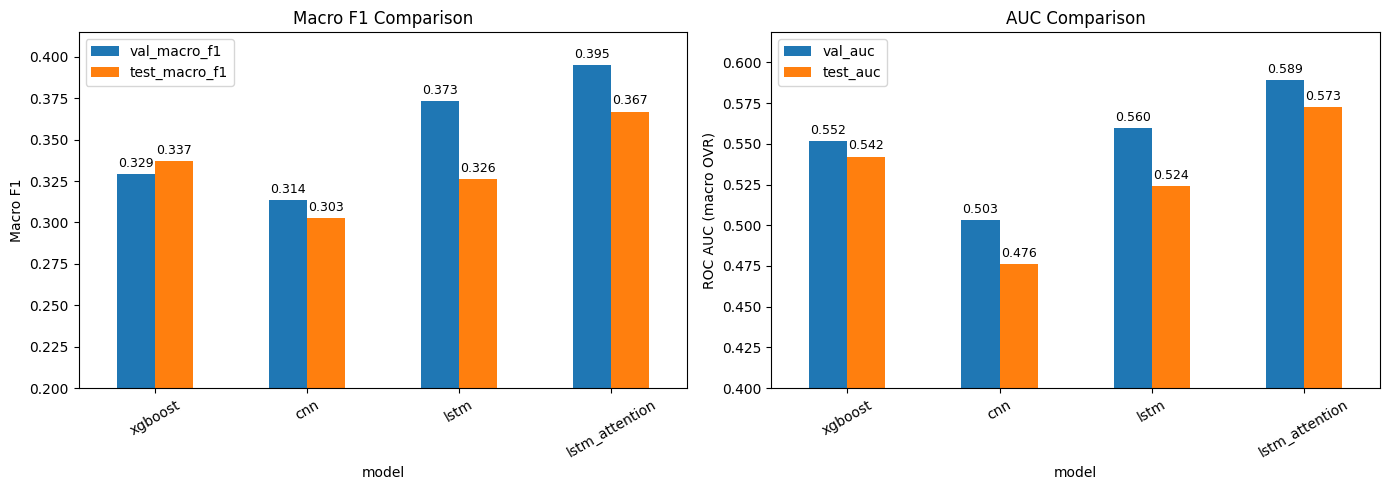
\includegraphics[width=0.9\linewidth]{figures/metrics_across_4_models.png}
    \caption{Model metrics across XGBoost, CNN, LSTM, and LSTM-attention on the selected TA+Sentiment dataset.}
\end{figure}

\begin{figure}[H]
    \centering
    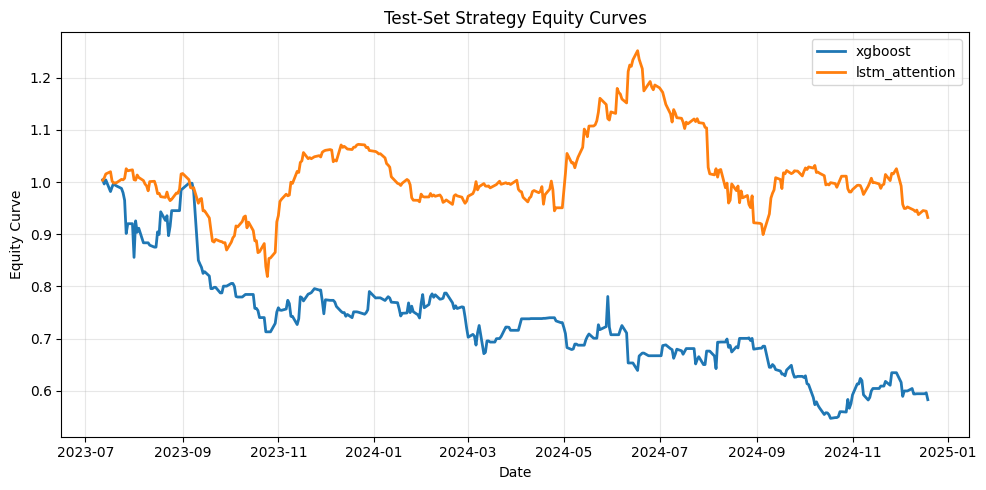
\includegraphics[width=0.78\linewidth]{figures/lstm_attention_vs_xgboost_equity.png}
    \caption{Backtest equity comparison between LSTM-attention and XGBoost on the selected TA+Sentiment dataset.}
\end{figure}

Under a common input representation, XGBoost remains a strong baseline, the CNN adds little, and the plain LSTM fails to surpass the tree benchmark, while LSTM-attention achieves the best classification metrics and carries this advantage through to downstream equity performance, supporting the hypothesis that cross-sectional interaction constitutes the missing modeling component.

\subsection{Confidence Filtering for Trading Execution}

Following model training, an additional decision layer is evaluated for the deep learning models. Rather than executing a trade on every predicted class, the strategy executes only when the maximum softmax probability exceeds a specified threshold; otherwise the model defaults to HOLD. This confidence filter modifies execution without requiring any retraining of the classifier.

The filter yields a material improvement in risk-adjusted performance. For the LSTM, a threshold of 0.50 reduces the number of trades from 228 to 48, increases the Sharpe ratio from 0.84 to 1.40, and improves total return. For the Transformer, filtering at 0.60 improves total return and reduces maximum drawdown to $-5.9\%$. These results indicate that confidence filtering operates as a simple yet effective execution overlay: once the predictive model is trained, additional selectivity at the decision stage can improve portfolio quality without modifying the underlying classifier.

\begin{table}[H]
    \centering
    \scriptsize
    \resizebox{\linewidth}{!}{
    \begin{tabular}{lcccc}
        \toprule
        Strategy & Total Return & Sharpe & Max Drawdown & Trades \\
        \midrule
        Buy \& Hold & +50.4\% & 1.36 & -18.2\% & 10 \\
        LSTM (no filter) & +11.4\% & 0.84 & -9.7\% & 228 \\
        LSTM, conf $\geq 0.50$ & +17.9\% & 1.40 & -7.1\% & 48 \\
        Transformer (no filter) & +8.4\% & 0.54 & -10.5\% & 179 \\
        Transformer, conf $\geq 0.60$ & +15.7\% & 1.17 & -5.9\% & 44 \\
        \bottomrule
    \end{tabular}
    }
    \caption{Trading results before and after confidence filtering for the deep models.}
\end{table}

\section{Exploratory Study: Factor Engineering and Alpha Mining}

Alongside the main modeling work, an exploratory study examines whether the input feature space itself can be enriched through automated factor discovery, rather than through further modification of the downstream classifier.

The methodology combines symbolic formula generation with reinforcement learning. A decoder-only Transformer autoregressively generates factor formulas in prefix notation, while a stack-based evaluator computes each generated formula exactly. The search objective integrates performance and stability criteria, including the K-ratio and ICIR, so that mined factors are both predictive and financially meaningful. The procedure preserves the interpretability of the discovered factors rather than treating feature construction as a black-box operation.

The exploratory results indicate that mined factors provide incremental value relative to an OHLCV-only baseline. The treatment model incorporating mined factors exhibits improvements in recall, F1 score, win rate, and Sharpe ratio within the reported experiment. Although this setup is not strictly comparable to the ten-stock architecture evaluation, the findings suggest a promising direction for future work in which enriched factor construction may be combined with the main modeling pipeline.

\begin{table}[H]
    \centering
    \scriptsize
    \resizebox{\linewidth}{!}{
    \begin{tabular}{lccccccc}
        \toprule
        Model & Accuracy & Precision & Recall & F1 & AUC-ROC & AUC-PR & Brier \\
        \midrule
        Control (OHLCV) & 0.5136 & 0.5625 & 0.4800 & 0.5180 & 0.5104 & 0.5517 & 0.2500 \\
        Treatment (OHLCV+Factors) & 0.4936 & 0.5313 & 0.5933 & 0.5606 & 0.4712 & 0.5301 & 0.2502 \\
        \bottomrule
    \end{tabular}
    }
    \caption{Classification metrics reported for the factor-mining approach.}
\end{table}

\begin{table}[H]
    \centering
    \scriptsize
    \resizebox{\linewidth}{!}{
    \begin{tabular}{lcccccccc}
        \toprule
        Model & Total Ret. & Ann. Ret. & Volatility & Sharpe & Max DD & Calmar & Win Rate & Trades \\
        \midrule
        Control (OHLCV) & -6.91\% & -3.22\% & 20.07\% & -0.161 & -25.70\% & -0.125 & 35.20\% & 273 \\
        Treatment (OHLCV+Factors) & -4.00\% & -1.85\% & 21.77\% & -0.085 & -33.19\% & -0.056 & 41.27\% & 179 \\
        \bottomrule
    \end{tabular}
    }
    \caption{Financial backtest metrics reported for the factor-mining approach.}
\end{table}

\section{Conclusion}

The project contributes at two principal levels, supplemented by an exploratory extension. The data-construction stage establishes the alignment, cleaning, and transformation of raw technical, sentiment, and fundamental sources into usable daily features. The model-design stage then advances from a strong tabular baseline to a sequence model augmented with cross-sectional interaction, with the ablation results showing that data combination is consequential and that distinct architectures favor different feature blocks, and the architecture results showing that both temporal structure and contemporaneous cross-sectional interaction are material, with LSTM-attention achieving the strongest performance on the selected TA+Sentiment dataset. The confidence-filtering analysis further demonstrates that execution-stage refinements can improve portfolio quality even when the classifier is held fixed.

The exploratory factor-mining study enriches the input space with interpretable alpha factors discovered via automated search and points toward a natural extension of the main pipeline: integrating the stronger downstream architecture with an enriched factor set and subsequently applying confidence-aware execution to the combined system.

\end{document}
